\documentclass[11pt,professionalfont,aspectratio=43]{beamer}

% Assets
\usepackage[czech]{babel}				% Jazyk
\usepackage[a-2u]{pdfx}				    % Kopírování z pdfka
\usepackage{tikz}						% Schémata automatů
\usetikzlibrary{shadows, shadows.blur, shapes.geometric, arrows, positioning, overlay-beamer-styles, patterns, shadings, shapes.callouts}
% \usetikzlibrary{arrows}
\usepackage{pgfplots}
% \pgfplotsset{compat=1.15}
% \usepackage{mathrsfs}
\usepackage[export]{adjustbox}

\usepackage[T1]{fontenc}
\usefonttheme[onlymath]{serif}
% \usepackage{newtxmath}
\usepackage{pxfonts}
\usepackage{slantsc}
% \usepackage{varwidth}

\usepackage[linesnumbered,ruled,vlined]{algorithm2e}                % Pseudokód algoritmů
\usepackage[utf8]{inputenc}
% \usepackage{textcomp}
\usepackage{hyperref}
\usepackage{fancybox}

%%% FONTS
% \usefonttheme{serif}
% \usepackage{lmodern}
\usepackage{helvet}

\hypersetup{%
    pdfencoding=auto,
    pdfauthor={\insertauthor},
    pdftitle={\insertsubtitle}
}
\usepackage{float}
\usepackage{csquotes}					% české uvozovky
\usepackage{enumerate}					% enumerate environment
\usepackage{indentfirst}
\usepackage{tcolorbox}                  % Fancy boxíky
\usepackage{mathtools}
\usepackage{pifont}
\usepackage{cancel}
\usepackage{subcaption}
\usepackage{soul}
\usepackage{makecell}                   % Zalomení v buňce tabulky
\usepackage{xcolor}
\usepackage{graphicx}
\usepackage{tabularx}
\usepackage{amsmath}
\usepackage{amsthm}
\usepackage{colortbl}                   % Barvení buněk v tabulce
\usepackage{multicol}                   % Rozdělení obsahu do sloucpů

\usepackage{listings}                   % Úryvky z kódu
\definecolor{maroon}{rgb}{0.5,0,0}
\definecolor{forestgreen}{rgb}{0.13, 0.55, 0.13}

% \lstdefinelanguage{XML}
% {
%   basicstyle=\ttfamily,
%   morestring=[s]{"}{"},
%   morecomment=[s]{?}{?},
%   morecomment=[s]{!--}{--},
%   commentstyle=\color{forestgreen},
%   moredelim=[s][\color{black}]{>}{<},
%   moredelim=[s][\color{red}]{\ }{=},
%   stringstyle=\color{blue},
%   identifierstyle=\color{maroon}
% }
% Colors

\def\maincolR{0} % červená složka (0–255)
\def\maincolG{83} % zelená složka
\def\maincolB{120} % modrá složka
\definecolor{maincolor}{HTML}{8B00B5}

% \pgfmathtruncatemacro{\authorfooterbgR}{1*\maincolR}
% \pgfmathtruncatemacro{\authorfooterbgG}{1*\maincolG}
% \pgfmathtruncatemacro{\authorfooterbgB}{1*\maincolB}
% \definecolor{authorfooterbg}{RGB}{\authorfooterbgR,\authorfooterbgG,\authorfooterbgB}

% \pgfmathtruncatemacro{\titlefooterbgR}{0.722*\maincolR}   
% \pgfmathtruncatemacro{\titlefooterbgG}{0.974*\maincolG}   
% \pgfmathtruncatemacro{\titlefooterbgB}{0.739*\maincolB}
% \definecolor{titlefooterbg}{RGB}{\titlefooterbgR,\titlefooterbgG,\titlefooterbgB}

% Beamer theme
\colorlet{themecolor}{maincolor}
\colorlet{authorfooterbg}{maincolor}
\definecolor{titlefooterbg}{HTML}{9471B0}
\definecolor{titlefooterfg}{HTML}{000000}
\colorlet{titlecolorfg}{maincolor}
\definecolor{titleboxbg}{HTML}{E7E7E7}
\definecolor{datefooterbg}{HTML}{E3E3E3}
\colorlet{titleframeboxcolor}{maincolor}

% Background gradient
\definecolor{gradMiddle}{RGB}{212,248,255}
\definecolor{gradEnd}{RGB}{114,231,255}

% Block theme
\definecolor{blocktitlebg}{HTML}{F0DFA9}
\definecolor{blocktitlefg}{HTML}{957300}
\definecolor{blockbodybg}{HTML}{F5F0DF}

\definecolor{alertblockbodybg}{HTML}{FFE4E4}
\definecolor{alertblocktitlebg}{HTML}{ECA4A4}
\definecolor{alertblocktitlefg}{HTML}{B11313}

\definecolor{exampleblockbodybg}{HTML}{DAF0DA}
\definecolor{exampleblocktitlebg}{HTML}{BBE0BB}
\definecolor{exampleblocktitlefg}{HTML}{257A25}

\definecolor{mathfg}{HTML}{00185E}

\colorlet{bulletbg}{maincolor}
% \definecolor{bulletbg}{HTML}{}

% Beamer theme
\usetheme{Madrid}
\usecolortheme{seahorse}
% \useoutertheme[subsection=false]{miniframes}

\usecolortheme[named=themecolor]{structure}
\setbeamertemplate{frame numbering}[fraction]
\setbeamertemplate{navigation symbols}{}
\setbeamercovered{invisible}

% Header/footer
\setbeamercolor{author in head/foot}{bg=authorfooterbg,fg=white}
\setbeamercolor{title in head/foot}{bg=titlefooterbg,fg=titlefooterfg}
\setbeamercolor{date in head/foot}{bg=datefooterbg,fg=black}
% \setbeamercolor{title}{bg=datefooterbg}
% \setbeamercolor{title}{fg=titlecolorfg}
\setbeamerfont{title}{series=\bfseries}
\setbeamercolor{frametitle}{bg=datefooterbg}
% \setbeamercolor{section in head/foot}{bg=red,fg=cyan}
% \setbeamercolor{subsection in head/foot}{bg=blue,fg=yellow}

% Table of contents
\setbeamercolor{section in toc}{fg=black}
\setbeamercolor{subsection in toc}{fg=red}
\setbeamercolor{section number projected}{fg=black}

% Blocks
\setbeamertemplate{blocks}[rounded][shadow=true]

\setbeamercolor{block title}{bg=blocktitlebg, fg=blocktitlefg}
\setbeamercolor{block body}{parent=normal text,use=block title,bg=blockbodybg}

\setbeamercolor{block body alerted}{bg=alertblockbodybg}
\setbeamercolor{block title alerted}{bg=alertblocktitlebg,fg=alertblocktitlefg}

\setbeamercolor{block body example}{bg=exampleblockbodybg}
\setbeamercolor{block title example}{bg=exampleblocktitlebg,fg=exampleblocktitlefg}

% Math
\setbeamercolor{math text}{fg=mathfg}

% Itemize a enumerate
\setbeamertemplate{itemize items}[circle]
\setbeamertemplate{enumerate items}[circle]
\setbeamercolor{itemize item}{fg=bulletbg,bg=white}
\setbeamercolor{itemize subitem}{fg=bulletbg,bg=white}
\setbeamercolor{itemize subsubitem}{fg=bulletbg,bg=white}

\setbeamertemplate{enumerate items}[circle]
\setbeamercolor{item projected}{bg=bulletbg}

% Titlepage
\defbeamertemplate*{title page}{customized}[1][]
{
    \vbox{}%
    \vfill%
    \begin{centering}
        \begin{tikzpicture}
            \node[thick, rectangle, rounded corners=5mm, drop shadow={shadow xshift=0mm, shadow yshift=2mm, opacity=0.2, blur shadow, shadow blur steps=10}, inner sep=5mm, fill=titleboxbg, fill opacity=1] {%
                {\usebeamerfont{title}\textcolor{titlecolorfg}{\inserttitle}\par}%
            };
        \end{tikzpicture}
        \vskip1em\par%
        \ifx\insertsubtitle\@empty%
        \else%
            {\usebeamerfont{subtitle}\insertsubtitle\par}%
        \fi%
        \vskip1em\par%
        \ifx\insertauthor\@empty%
        \else%
            {\usebeamerfont{author}\insertauthor}\\%
            \texttt{\email}
        \fi
        \vskip0.3em\par%
        % \ifx\insertinstitute\@empty%
        % \else%
        %     {\usebeamerfont{institute}\insertinstitute\par}%
        % \fi%
        \vskip1em\par%
        \ifx\inserttitlegraphic\@empty%
        \else%
            \vskip1em\par%
            \inserttitlegraphic\par%
        \fi%
        \vskip1em\par%
        \ifx\insertdate\@empty%
        \else%
            {\usebeamerfont{date}\insertdate\par}%
        \fi%
    \end{centering}%
    \vfill%
}
% Enumerate
%\setlist[enumerate]{topsep=0pt,itemsep=-1ex,partopsep=1ex,parsep=1ex,label=(\arabic*)}

\MakeOuterQuote{"}

%%% Makra pro definice, věty, tvrzení, příklady, ... (vyžaduje baliček amsthm)

\theoremstyle{plain}
\newtheorem{thm}{Věta}[section]
\newtheorem{lem}[theorem]{Lemma}
\newtheorem{prop}[theorem]{Tvrzení}
\newtheorem{cor}[theorem]{Důsledek}
\newtheorem*{prop*}{Tvrzení}

\theoremstyle{definition}
\newtheorem{define}[theorem]{Definice}
% \newtheorem{example}[theorem]{Příklad}
% \newtheorem{remark}[theorem]{Poznámka}
% \newtheorem{convention}[theorem]{Úmluva}
% \newtheorem{denoting}[theorem]{Značení}

\newenvironment{defblock}[1][]{
  \begin{block}{\ifthenelse{\equal{#1}{}}
  {Definice}
  {Definice (#1)}}
}{\end{block}}
\newenvironment{thmblock}[1][]{
  \begin{block}{\ifthenelse{\equal{#1}{}}
  {Věta}
  {Věta (#1)}}
}{\end{block}}
\newenvironment{corblock}[1][]{
  \begin{block}{\ifthenelse{\equal{#1}{}}
  {Důsledek}
  {Důsledek (#1)}}
}{\end{block}}
\newenvironment{propblock}[1][]{
  \begin{block}{\ifthenelse{\equal{#1}{}}
  {Tvrzení}
  {Tvrzení (#1)}}
}{\end{block}}
\newenvironment{exblock}[1][]{
  \begin{exampleblock}{\ifthenelse{\equal{#1}{}}
  {Příklad}
  {Příklad (#1)}}
}{\end{exampleblock}}


% Colors
\definecolor{lightblue}{HTML}{009AD4}
\definecolor{lightgreen}{HTML}{68FF00}
\definecolor{darkgreen}{HTML}{00B600}
\definecolor{darkblue}{HTML}{0265b3}
\definecolor{darkred}{HTML}{DA0707}
\definecolor{lightred}{HTML}{FF5100}
\definecolor{orange}{HTML}{FFE000}
\definecolor{codeblue}{HTML}{007eed}
\definecolor{codegreen}{rgb}{0,0.6,0}
\definecolor{codegray}{rgb}{0.5,0.5,0.5}
\definecolor{codebeige}{HTML}{D4A000}
\definecolor{codepink}{HTML}{FF0055}
\definecolor{backcolour}{rgb}{0.95,0.95,0.92}

\definecolor{decproblemtitlefg}{HTML}{957300}
\definecolor{decproblembg}{HTML}{F5F0DF}

\definecolor{timportantboxcolor}{HTML}{A97100}
\definecolor{talertboxcolor}{HTML}{B70000}
\definecolor{tnoticeboxcolor}{HTML}{159C00}
\definecolor{tinfoboxcolor}{HTML}{004DFF}

\newcommand{\markred}[1]{\textcolor{lightred}{#1}}
\newcommand{\markdarkred}[1]{\textcolor{darkred}{#1}}
\newcommand{\markgreen}[1]{\textcolor{lightgreen}{#1}}
\newcommand{\markdarkgreen}[1]{\textcolor{darkgreen}{#1}}
\newcommand{\markorange}[1]{\textcolor{orange}{#1}}
\newcommand{\markblue}[1]{\textcolor{lightblue}{#1}}
\newcommand{\markdarkblue}[1]{\textcolor{darkblue}{#1}}

% Math mode settings
% \AtBeginDocument{
%     \setlength{\abovedisplayskip}{3pt}
%     \setlength{\belowdisplayskip}{-4pt}
% }

% Inline images
\newcommand{\inlineimgscale}{1.1}

% X and check mark
\newcommand{\cmark}{\markgreen{\ding{51}}}
\newcommand{\xmark}{\markred{\ding{55}}}

% Math
\newcommand{\R}{\mathbb{R}}
\newcommand{\C}{\mathbb{C}}
\newcommand{\N}{\mathbb{N}}
\newcommand{\Z}{\mathbb{Z}}
\newcommand{\Q}{\mathbb{Q}}

\newcommand{\T}[1]{#1^\top}                     % Tranpozice matice
\newcommand{\compl}[1]{#1^\complement}
\newcommand{\mapping}[3]{#1:#2 \rightarrow #3}
\newcommand{\mapto}[3]{#1:#2 \mapsto #3}
\newcommand{\set}[1]{\left\{#1\right\}}
\newcommand{\powset}{\mathcal{P}}
\newcommand{\code}[1]{\langle#1\rangle}
\DeclareMathOperator*{\argmin}{arg\,min}
\DeclareMathOperator*{\argmax}{arg\,max}

% Statistika a AI
\newcommand{\average}[1]{\overline{#1}}
\DeclareMathOperator{\median}{med}
\DeclareMathOperator{\Var}{var}
\DeclareMathOperator{\Cov}{cov}
\DeclareMathOperator{\MSE}{MSE}
\DeclareMathOperator{\SSE}{SSE}

\DeclareMathOperator{\TP}{TP}
\DeclareMathOperator{\TN}{TN}
\DeclareMathOperator{\FP}{FP}
\DeclareMathOperator{\FN}{FN}
\DeclareMathOperator{\Accuracy}{Acc}
\DeclareMathOperator{\Precision}{Prec}
\DeclareMathOperator{\Recall}{Rec}
\DeclareMathOperator{\Fscore}{F}
\DeclareMathOperator{\Gini}{Gini}

\DeclareMathOperator{\mspan}{span}
\DeclareMathOperator{\mrank}{rank}
\DeclareMathOperator{\tg}{tg}
\DeclareMathOperator{\id}{id}
\DeclareMathOperator{\dom}{dom}
\DeclareMathOperator{\rng}{rng}
\renewcommand{\emptyset}{\varnothing}
\newcommand{\binary}[1]{\ensuremath{\left\langle #1\right\rangle}_B}

% DFS in and out lists
\DeclareMathOperator{\inlist}{in}
\DeclareMathOperator{\outlist}{out}
% \DeclareMathOperator{\lowlist}{low}
\DeclareMathOperator{\key}{key}

% A* macro
\newcommand{\Astar}{$\textcolor{black}{\textup{A}^{*}}$}

% Complexity classes
\DeclareMathOperator{\classP}{P}
\DeclareMathOperator{\classNP}{NP}
\DeclareMathOperator{\classTime}{TIME}
\DeclareMathOperator{\classNTime}{NTIME}
\DeclareMathOperator{\classSpace}{SPACE}
\DeclareMathOperator{\classNSpace}{NSPACE}

\DeclareMathOperator{\SAT}{SAT}
\DeclareMathOperator{\THREESAT}{3-SAT}
\DeclareMathOperator{\UNSAT}{UNSAT}
\DeclareMathOperator{\NZMNA}{NzMna}
\DeclareMathOperator{\KLIKA}{Klika}
\DeclareMathOperator{\ROZVRH}{Rozvrh}
\DeclareMathOperator{\SUDOKU}{Sudoku}
\newcommand{\HALT}{\ensuremath{\textsc{Halt}}}
\newcommand{\FACTOR}{\ensuremath{\textsc{Factor}}}

\DeclareMathOperator{\regex}{RegE}

%%% Barevné boxíky (notice / info / important / alert)
%
% Šířka boxu se nezadává ručně -- box se přizpůsobí šířce svého obsahu.
% Obsah se vysází do prostředí varwidth, takže krátký text zůstane na
% jednom řádku; delší text se zalomí, nejvýše však na šířku \linewidth
% (tj. \textwidth mimo sloupce a minipage). Pokud je titulek širší než
% obsah, řídí šířku boxu titulek.

\newsavebox{\tboxcontentbox}
\newsavebox{\tboxtitlebox}
\newlength{\tboxwidth}
\newlength{\tboxpadding}

% Geometrie boxu (musí odpovídat stylu tautobox níže):
% 2 * (boxrule + boxsep + left)
\setlength{\tboxpadding}{\dimexpr 0.5mm+1mm+4mm\relax}
\setlength{\tboxpadding}{2\tboxpadding}

\tcbset{tautobox/.style={boxrule=0.5mm, boxsep=1mm, left=4mm, right=4mm,
                         fonttitle=\bfseries}}

% Začátek sběru obsahu do boxu
\newcommand{\tboxcollect}{%
  \begin{lrbox}{\tboxcontentbox}%
    \begin{varwidth}{\dimexpr\linewidth-\tboxpadding\relax}%
}

% Ukončení sběru a výpočet výsledné šířky
% #1 = titulek (pro měření; prázdný u variant bez titulku)
\newcommand{\tboxmeasure}[1]{%
    \end{varwidth}%
  \end{lrbox}%
  \sbox{\tboxtitlebox}{\bfseries #1}%
  \setlength{\tboxwidth}{\wd\tboxcontentbox}%
  \ifdim\wd\tboxtitlebox>\tboxwidth
    \setlength{\tboxwidth}{\wd\tboxtitlebox}%
  \fi
  \addtolength{\tboxwidth}{\tboxpadding}%
  \ifdim\tboxwidth>\linewidth
    \setlength{\tboxwidth}{\linewidth}%
  \fi
}

% Vysázení boxu s titulkem: #1 = barva, #2 = titulek
\newcommand{\tboxrenderbox}[2]{%
  \tboxmeasure{#2}%
  \begin{center}%
    \begin{tcolorbox}[tautobox, colback=#1!15, colframe=#1,
                      title={#2}, width=\tboxwidth]
      \usebox{\tboxcontentbox}%
    \end{tcolorbox}%
  \end{center}%
}

% Vysázení boxu bez titulku: #1 = barva
\newcommand{\tboxrenderframe}[1]{%
  \tboxmeasure{}%
  \begin{center}%
    \begin{tcolorbox}[tautobox, colback=#1!15, colframe=#1,
                      width=\tboxwidth]
      \usebox{\tboxcontentbox}%
    \end{tcolorbox}%
  \end{center}%
}

% Poznámky (notice)
\newenvironment{tnoticebox}[1]{%
  \def\tboxtitletext{#1}\tboxcollect
}{%
  \tboxrenderbox{tnoticeboxcolor}{\tboxtitletext}%
}

\newenvironment{tnoticeframe}{%
  \tboxcollect
}{%
  \tboxrenderframe{tnoticeboxcolor}%
}

% Informační bloky (info)
\newenvironment{tinfobox}[1]{%
  \def\tboxtitletext{#1}\tboxcollect
}{%
  \tboxrenderbox{tinfoboxcolor}{\tboxtitletext}%
}

\newenvironment{tinfoframe}{%
  \tboxcollect
}{%
  \tboxrenderframe{tinfoboxcolor}%
}

% Důležité bloky (important)
\newenvironment{timportantbox}[1]{%
  \def\tboxtitletext{#1}\tboxcollect
}{%
  \tboxrenderbox{timportantboxcolor}{\tboxtitletext}%
}

\newenvironment{timportantframe}{%
  \tboxcollect
}{%
  \tboxrenderframe{timportantboxcolor}%
}

% Varovné bloky (alert)
\newenvironment{talertbox}[1]{%
  \def\tboxtitletext{#1}\tboxcollect
}{%
  \tboxrenderbox{talertboxcolor}{\tboxtitletext}%
}

\newenvironment{talertframe}{%
  \tboxcollect
}{%
  \tboxrenderframe{talertboxcolor}%
}

% Decision problem
\newcommand{\decproblem}[3]{
    \begin{center}
        \begin{minipage}{.9\textwidth}
            \begin{table}[!htbp]
                \centering
                \bgroup
                \def\arraystretch{1.8}
                \begin{tabularx}{\textwidth}{|rX|}
                \hline
                \rowcolor{decproblembg} \multicolumn{2}{|c|}{\textcolor{decproblemtitlefg}{\textsc{#1}}} \\ \hline
                \markdarkred{\textbf{Vstup:}} & #2                \\ \hline
                \rowcolor{decproblembg} \markdarkred{\textbf{Otázka:}} & #3               \\ \hline
                \end{tabularx}
                \egroup
            \end{table}
        \end{minipage}
    \end{center}
}
\newcommand{\bigO}{\mathcal{O}}

% TODO
\newcommand{\todo}[1]{\textcolor{red}{(\noindent TODO: #1.)}}


\newcommand{\hlcode}[1]{\colorbox{red}{#1}}

% Algorithms
\numberwithin{algocf}{section}
\renewcommand{\algorithmcfname}{Algoritmus}
\SetKwInput{KwIn}{Vstup}
\SetKwInput{KwOut}{Výstup}
\SetKwProg{Function}{Funkce}{}{end}
\setlength{\algomargin}{25pt}
\renewcommand{\thealgocf}{}     % Vypnutí číslování algoritmů

% Definice stylů pro uzly
\tikzstyle{startstop} = [rectangle, rounded corners, minimum width=1.5cm, minimum height=0.5cm,text centered, draw=black, fill=red!30]
\tikzstyle{process}   = [rectangle, minimum width=1.5cm, minimum height=0.5cm, text centered, draw=black, fill=orange!30]
\tikzstyle{decision}  = [diamond, aspect=2, text centered, draw=black, fill=green!30]
\tikzstyle{arrow}     = [thick,->,>=stealth]

\tikzstyle{vertex}    = [thick, draw, circle, minimum size=4mm, inner sep=1pt, outer sep=1pt, align=center]
\tikzstyle{vertexplain}    = [minimum size=4mm, inner sep=1pt, outer sep=1pt, align=center]
\tikzstyle{verteximg}    = [draw, circle, minimum size=4mm, inner sep=0pt, outer sep=1pt, align=center, clip]
\tikzstyle{verteximgplain}    = [minimum size=4mm, inner sep=0pt, outer sep=1pt, align=center]
\tikzstyle{task}    = [draw, rounded corners=2pt, minimum width=14mm, minimum height=8mm, inner sep=2pt, align=center]

\tikzstyle{edge}    = [thick,>=stealth]
\tikzstyle{diredge}    = [thick, ->, >=stealth]

%% Automaty
\tikzstyle{state}=[%
    draw,
    circle,
    thick,
    minimum size=10mm,
    inner sep=0pt,
    outer sep=0pt
]

\tikzstyle{acceptstate}=[%
    state,
    double,
    double distance=1pt
]

\tikzstyle{transition}=[%
    ->,
    >=stealth,
    thick
]

\newcommand<>{\state}[4][]{%
    \node#5[state,#1] (#2) at #3 {#4};
}

\newcommand<>{\acceptingstate}[4][]{%
    \node#5[acceptstate,#1] (#2) at #3 {#4};
}

\newcommand<>{\transitionarrow}[5][]{%
    \path#6 (#2) edge[transition,#1] node[#3] {#4} (#5);
}

\newcommand<>{\initialstate}[6][]{%
    \node#7[state,#1] (#2) at #3 {#4};
    \draw#7[transition] #5 -- (#2.#6);
}

%%%%%

% Frames
\newcommand{\tableofcontentsframe}{
    \begin{frame}{Obsah}
        \tableofcontents
    \end{frame}
}

% \definecolor{boxcolor}{HTML}{00820a}
\newcommand{\titleframe}[1]{%
  \begin{frame}[plain]
    \begin{tikzpicture}[remember picture, overlay]
      \node at (current page.center)
        [draw=titleframeboxcolor, line width=1pt,
         inner xsep=10mm, inner ysep=4mm, rounded corners=2mm,
         text width=0.8\textwidth, align=center,
         execute at begin node=\setlength{\baselineskip}{2.2em}]
        {\Huge\markred{#1}\normalfont};
    \end{tikzpicture}
  \end{frame}
  \addtocounter{framenumber}{-1}%
}

\newenvironment{titleframeenv}[1]{
    \begin{frame}[plain]
        \begin{tcolorbox}[colback=white,boxrule=1pt]
            \begin{center}
                \Huge\markred{#1}\normalfont
            \end{center}
        \end{tcolorbox}
}{\addtocounter{framenumber}{-1}\end{frame}}

\newcommand{\icon}[1]{
  \includegraphics[height=\fontcharht\font`\B]{#1}
}

% Obrázek, který se vždy vejde na snímek. Adjustbox jej v případě potřeby
% zmenší tak, aby nepřesáhl šířku textu ani zadanou část výšky snímku; díky
% tomu sedí sazba ve všech používaných poměrech stran (4:3, 16:9 i 16:10).
% Volitelným argumentem je maximální výška (výchozí 0.68\textheight), povinným
% cesta k souboru s obrázkem (TikZ zdroj vkládaný přes \input).
\newcommand{\obrazek}[2][0.68\textheight]{%
    \begin{figure}
        \centering
        \begin{adjustbox}{max width=\linewidth, max totalheight=#1, center}
            \input{#2}
        \end{adjustbox}
    \end{figure}%
}

% Totéž pro rastrové či vektorové obrázky vkládané přes \includegraphics.
\newcommand{\obrazekgrf}[2][0.68\textheight]{%
    \begin{figure}
        \centering
        \includegraphics[width=\linewidth, max totalheight=#1, center]{#2}
    \end{figure}%
}

% Závěrečný snímek se seznamem zdrojů. Prvním (volitelným) argumentem je název
% sekce i snímku, druhým čárkou oddělený seznam klíčů z ../assets/literatura.bib.
% Citace se sázejí podle ČSN ISO 690, v pořadí, v jakém jsou klíče uvedeny.
\newcommand{\zdrojeframe}[2][Zdroje]{%
    \section{#1}
    \nocite{#2}%
    \begin{frame}[allowframebreaks]{#1}
        \printbibliography[heading=none]
    \end{frame}
}
\input{../assets/listing.tex}

\def\presentationtitle{Neuronové sítě}

\begin{document}

\title[\presentationtitle]{\textsc{Teoretická informatika}}
\subtitle{\presentationtitle}
\author{David Weber}
\def\email{weber3@spsejecna.cz}
\institute{SPŠE Ječná}
\date{%
    Rok 
    \pgfmathsetmacro{\firstyear}{ifthenelse(\month<9, \year-1, \year)}%
    \pgfmathsetmacro{\secondyear}{ifthenelse(\month<9, \year, \year+1)}%
    \pgfmathtruncatemacro{\secondyearlasttwo}{mod(\secondyear,100)}%
    \pgfmathprintnumber[fixed,precision=0,zerofill,1000 sep={}]{\firstyear}/%
    \pgfmathprintnumber[fixed,precision=0,zerofill,1000 sep={}]{\secondyearlasttwo}%
}
\titlegraphic{\includegraphics[width=0.25\textwidth]{../images/SPSE-Jecna_Logo.pdf}}

\begin{frame}[plain]
    \titlepage
\end{frame}

\section{Úvod}

\titleframe{Úvod do neuronových sítí}

\subsection{Motivace}

\begin{frame}{Proč neuronové sítě?}
    \pause
    \begin{columns}[T]
        \begin{column}{0.56\textwidth}
            \begin{itemize}
                \item V~předchozích prezentacích jsme viděli, že modely se mohou učit z~dat.
                \pause
                \item Některé vztahy v~datech jsou ale příliš složité pro jednoduchý lineární model.
                \pause
                \item Neuronové sítě umožňují skládat více jednoduchých výpočtů za sebou.
                \pause
                \item Díky tomu mohou modelovat i~složitější nelineární vztahy.
            \end{itemize}
        \end{column}

        \begin{column}{0.40\textwidth}
            \centering
            \begin{tikzpicture}[
                >=stealth,
                box/.style={
                    draw,
                    rounded corners=2mm,
                    minimum width=25mm,
                    minimum height=11mm,
                    align=center
                },
                arr/.style={
                    ->,
                    thick,
                    rounded corners=2mm
                },
                node distance=8mm,
                every node/.style={font=\small}
            ]
                \node[box] (data) {data};
                \node[box, below=of data] (model) {model};
                \node[box, below=of model] (zaver) {závěr};

                \draw[arr] (data) -- (model);
                \draw[arr] (model) -- (zaver);
            \end{tikzpicture}
        \end{column}
    \end{columns}

    \pause

    \begin{timportantbox}[0.94\textwidth]{Základní myšlenka}
        Neuronová síť je model složený z~mnoha jednoduchých výpočetních jednotek,
        jejichž propojení a~váhy se nastavují během učení.
    \end{timportantbox}

\end{frame}


\begin{frame}{Co již víme\dots}
    \pause
    \begin{tinfobox}[\textwidth]{Připomenutí}
        V~úlohách učení s~učitelem (anglicky
        \markdarkred{supervised learning}) pracujeme se statistickými soubory $\mathbf{X}_1,\mathbf{X}_2,\ldots,\mathbf{X}_p$
        a~se statistickým souborem očekávaných výstupů $\mathbf{Y}$.
    \end{tinfobox}

    \pause

    Pro \(i\)-tý datový záznam získáme vektor dat
    \[
        \mathbf{x}_i
        =
        (x_{i1},x_{i2},\ldots,x_{ip}),
    \]
    kterému odpovídá očekávaný výstup \(y_i\).

    \pause
    \vspace{2mm}
    \centering
    \begin{tikzpicture}[
        >=stealth,
        box/.style={
            draw,
            rounded corners=2mm,
            minimum width=25mm,
            minimum height=11mm,
            align=center
        },
        arr/.style={
            ->,
            thick,
            rounded corners=2mm
        },
        node distance=10mm,
        every node/.style={font=\small}
    ]
        \node[box] (input) {
            vektor dat\\
            \(\mathbf{x}_i\)
        };

        \node[box, right=of input] (model) {
            model
        };

        \node[box, right=of model] (output) {
            vypočtený výstup\\
            \(\hat{y}_i\)
        };

        \node[box, below=8mm of output] (expected) {
            očekávaný výstup\\
            \(y_i\)
        };

        \draw[arr] (input) -- (model);
        \draw[arr] (model) -- (output);
        \draw[arr] (expected) -- (output);
    \end{tikzpicture}

\end{frame}

\subsection{Biologický neuron}

\begin{frame}{Neuron jako biologická inspirace}
    \pause
    \begin{itemize}
        \item Neuron je buňka nervové soustavy, která zpracovává a~předává signály.
        \pause
        \item Signály přijímá pomocí dendritů.
        \pause
        \item Zpracovaný signál je veden dále axonem.
        \pause
        \item Ke komunikaci mezi neurony dochází pomocí synaptických spojů.
    \end{itemize}

    \pause

    \begin{timportantbox}[\textwidth]{Myšlenka pro informatiku}
        Biologický neuron slouží jako inspirace pro jednoduchý výpočetní model.
    \end{timportantbox}

\end{frame}

\begin{frame}{Schéma biologického neuronu}
    \centering
    \begin{tikzpicture}[
        >=stealth,
        arr/.style={
            ->,
            thick,
            rounded corners=2mm,
            red
        },
    ]
        
        \node at (0,0) {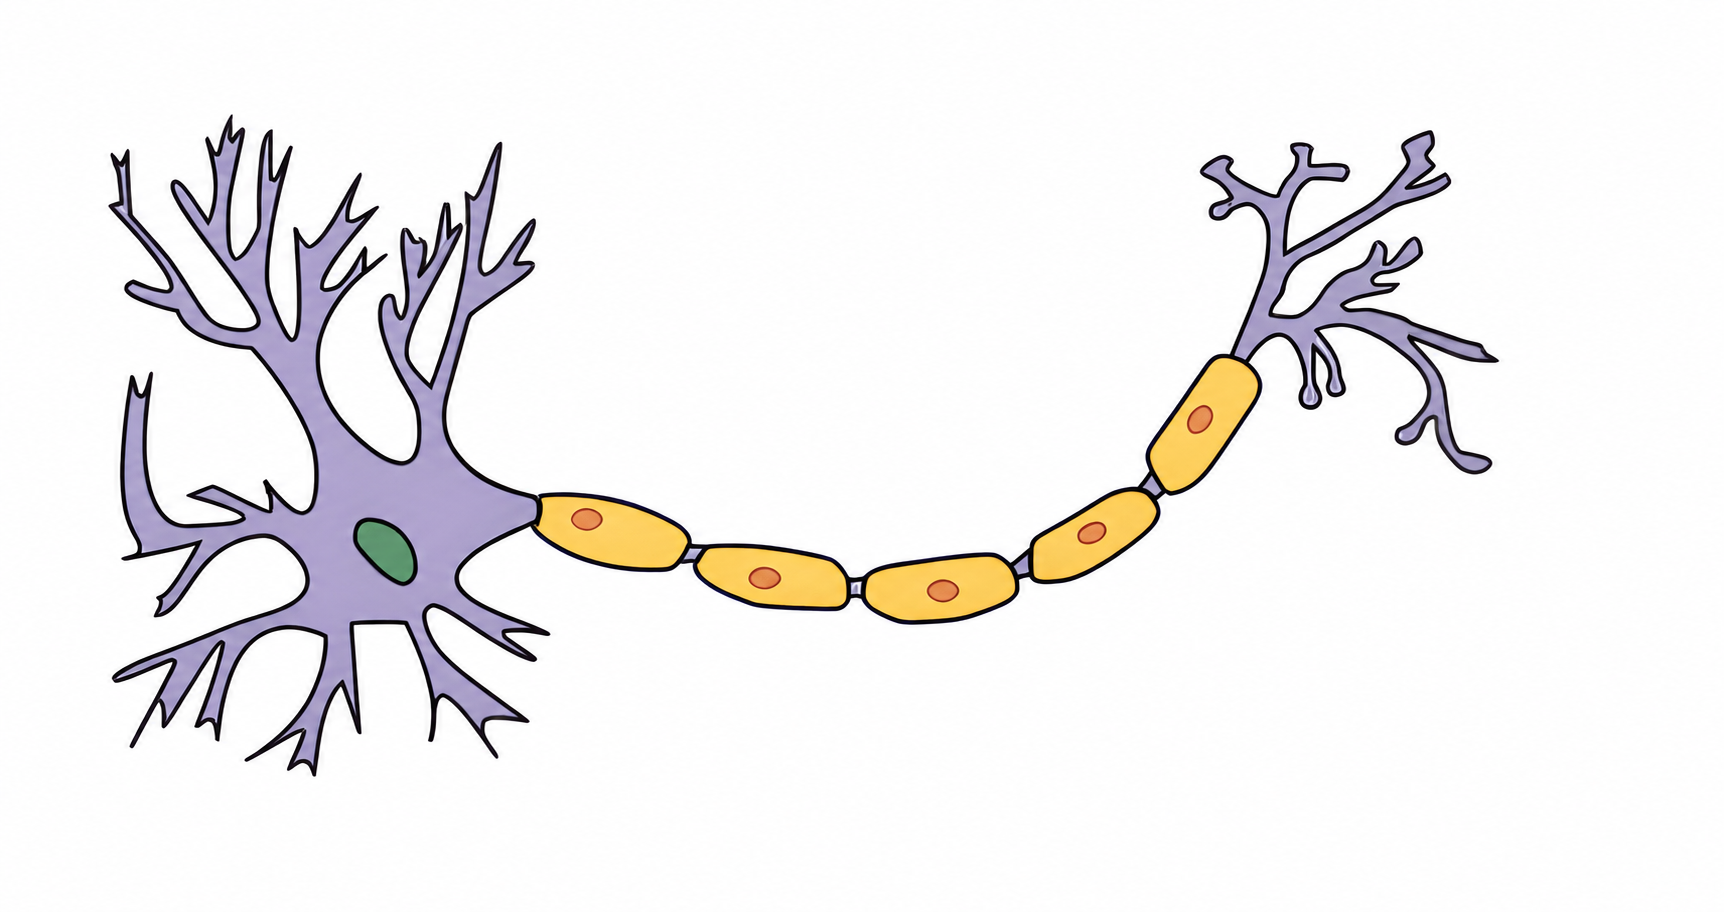
\includegraphics[width=12cm]{images/neuron.png}};

        % Dendrity
        \node (dentrites) at (-3,-3) {Dendrity};
        \draw[arr] (dentrites) -- (-3.5,-2);
        \draw[arr] (dentrites) -- (-2.7,-2);

        % Cell body
        \node (cellbody) at (-1.2,0.8) {Tělo buňky};
        \draw[arr] (cellbody) -- (-3,-0.3);

        % Axon trunk
        \node (cellbody) at (1,-2.5) {Axonové vlákno};
        \draw[arr] (cellbody) -- (0.7,-1.2);

        % Synapses
        \node (synapses) at (4.5,3) {Synapse};
        \draw[arr] (synapses) -- (3.2,2.1);
        \draw[arr] (synapses) -- (4,1);

    \end{tikzpicture}

    \begin{figure}
        \centering
        
    \end{figure}

\end{frame}

\subsection{Od biologie k modelu}

\begin{frame}{Od biologického neuronu k formálnímu neuronu}

    \begin{center}
    \begin{tikzpicture}[
        >=stealth,
        box/.style={
            draw,
            rounded corners=2mm,
            minimum width=25mm,
            minimum height=11mm,
            align=center
        },
        arr/.style={
            ->,
            thick,
            rounded corners=2mm
        },
        node distance=3mm,
        every node/.style={font=\small}
    ]

        \node[box] (inputs) {vstupní\\signály};
        \node[box, below=of inputs] (synstrength) {síla synaptických\\spojů};
        \node[box, below=of synstrength] (activation) {aktivace\\neuronu};
        
        \node[box, right=3cm of inputs] (inputsformal) {$x_1,\ldots,x_n$};
        \node[box, below=of inputsformal] (synstrengthformal) {$w_1,\ldots,w_n$};
        \node[box, below=of synstrengthformal] (activationformal) {$f$};

        \draw[arr] (inputs) -- (inputsformal);
        \draw[arr] (synstrength) -- (synstrengthformal);
        \draw[arr] (activation) -- (activationformal);

    \end{tikzpicture}
    \end{center}

    \pause

    \begin{timportantbox}[\textwidth]{Zjednodušení}
        Formální neuron nepopisuje biologické děje uvnitř buňky.
        Formální neuron popisuje jednoduchý výpočet: sečtení vážených vstupů
        a~rozhodnoutí o~výstupu.
    \end{timportantbox}

\end{frame}

\begin{frame}{Synaptický spoj jako váha}

    \begin{columns}[T]
        \begin{column}{0.48\textwidth}
            \begin{itemize}
                \pause
                \item Každý vstup může mít jiný význam.
                \pause
                \item Váha \(w_j\) určuje, jak silně vstup \(x_j\) ovlivňuje výstup neuronu.
                \pause
                \item Kladná váha výstup podporuje.
                \pause
                \item Záporná váha výstup potlačuje.
            \end{itemize}
        \end{column}
        \pause
        \begin{column}{0.48\textwidth}
            \centering
            \begin{tikzpicture}[
                >=stealth,
                box/.style={
                    draw,
                    rounded corners=2mm,
                    minimum width=8mm,
                    minimum height=8mm,
                    align=center
                },
                arr/.style={
                    ->,
                    thick,
                    rounded corners=2mm
                },
                node distance=9mm,
                every node/.style={font=\small}
            ]

                \node[box] (x1) at (0,1.2) {\(x_1\)};
                \node[box] (x2) at (0,0) {\(x_2\)};
                \node[box] (x3) at (0,-1.2) {\(x_3\)};

                \node[box, right=16mm of x2] (n) {neuron};
                \node[box, right=11mm of n] (y) {\(y\)};

                \draw[arr] (x1) -- node[above] {\(w_1\)} (n);
                \draw[arr] (x2) -- node[above] {\(w_2\)} (n);
                \draw[arr] (x3) -- node[below] {\(w_3\)} (n);
                \draw[arr] (n) -- (y);

            \end{tikzpicture}
        \end{column}
    \end{columns}

    \pause

    \begin{tnoticebox}[\textwidth]{Poznámka}
        V~neuronové síti nejsou váhy předem pevně dané.
        Síť se je snaží nastavit během učení.
    \end{tnoticebox}

\end{frame}

\subsection{Neuronová síť jako graf}

\begin{frame}{Neuronová síť jako graf}

    Neuronovou síť můžeme chápat jako orientovaný ohodnocený graf.
    Vrcholy představují neurony a~hrany představují spoje mezi nimi.
    \pause

    \vspace{3mm}

    \centering
    \begin{tikzpicture}[
        >=stealth,
        arr/.style={
            ->,
            thick,
            rounded corners=2mm
        },
        node distance=13mm,
        every node/.style={font=\small}
    ]

        \node[vertex] (x1) at (0,1.2) {\(x_1\)};
        \node[vertex] (x2) at (0,0) {\(x_2\)};
        \node[vertex] (x3) at (0,-1.2) {\(x_3\)};

        \node[vertex] (h1) at (2.4,0.7) {};
        \node[vertex] (h2) at (2.4,-0.7) {};

        \node[vertex] (y) at (4.8,0) {\(y\)};

        \foreach \x in {x1,x2,x3} {
            \foreach \h in {h1,h2} {
                \draw[arr] (\x) -- (\h);
            }
        }

        \draw[arr] (h1) -- (y);
        \draw[arr] (h2) -- (y);

        \node[below=3mm of x3] {vstupy};
        \node[below=8mm of h2] {neurony};
        \node[below=8mm of y] {výstup};

    \end{tikzpicture}

    \pause

    \begin{timportantframe}[\textwidth]
        Na rozdíl od jednoho neuronu může celá síť skládat více výpočtů
        dohromady. Právě tím získává větší vyjadřovací schopnost.
    \end{timportantframe}

\end{frame}

\section{Formální neuronová síť}

\titleframe{Formální neuronová síť}

\subsection{Formální neuron}

\begin{frame}{Formální neuron}
    \pause

    \centering
    \begin{tikzpicture}[
        node distance=10mm,
        every node/.style={font=\small}
    ]

        % Vstupy
        \node[vertex] (x1) at (0,1.5) {\(x_{i1}\)};
        \node[vertex] (x2) at (0,0.5) {\(x_{i2}\)};
        \node[vertexplain] (dots) at (0,-0.35) {\(\vdots\)};
        \node[vertex] (xp) at (0,-1.3) {\(x_{ip}\)};

        % Zpracování
        \node[task, minimum width=19mm, minimum height=12mm]
            (sum) at (3.0,0.1)
            {vážený\\součet};

        \node[task, minimum width=14mm, minimum height=12mm]
            (activation) at (5.2,0.1)
            {%
                \(\displaystyle f\)
            };

        \node[vertex]
            (output) at (7.0,0.1)
            {\(\hat{y}_i\)};

        % Bias
        \node[vertex]
            (bias) at (3.0,-1.7)
            {\(b\)};

        % Hrany od vstupů
        \draw[diredge]
            (x1) --
            node[pos=0.48, above, sloped] {\(w_1\)}
            (sum);

        \draw[diredge]
            (x2) --
            node[pos=0.48, above, sloped] {\(w_2\)}
            (sum);

        \draw[diredge]
            (xp) --
            node[pos=0.48, below, sloped] {\(w_p\)}
            (sum);

        % Bias
        \draw[diredge]
            (bias) -- (sum);

        % Výstupní část
        \draw[diredge]
            (sum) --
            node[above] {\(z_i\)}
            (activation);

        \draw[diredge]
            (activation) -- (output);

        % Popisky
        \node[vertexplain, below=5mm of xp]
            {vstupy};

        \node[vertexplain, below=5mm of activation]
            {přenosová funkce};

    \end{tikzpicture}

    \pause

    \begin{timportantframe}[\textwidth]
        Formální neuron nejprve spočítá vážený součet vstupů
        a~poté na něj aplikuje přenosovou funkci.
    \end{timportantframe}

\end{frame}

\begin{frame}{Výpočet formálního neuronu}
    \pause
    \begin{itemize}
        \item Pro \(i\)-tý datový záznam máme vektor
        \[
            \mathbf{x}_i
            =
            (x_{i1},x_{i2},\ldots,x_{ip}).
        \]\pause
        a~vstupní váhy neuronu $w_1,w_2,\ldots,w_p$.
        \item Z~toho spočítáme výstupní hodnotu
        \[
            \hat{y}_i=f\left(\sum_{j=1}^{p} w_j x_{ij}-\theta\right),
        \]
        kde
        \pause
        \begin{itemize}
            \item \(\theta\) je tzv. \markdarkred{bias}, který umožňuje posunout rozhodování neuronu a\pause
            \item $f$ je tzv. \markdarkred{aktivační funkce} (anglicky \markdarkred{activation function}, viz později).
        \end{itemize}
    \end{itemize}

\end{frame}


\begin{frame}{Váhy a~prahová hodnota}
    \pause
    \begin{itemize}
        \item Váha \(w_j\) určuje význam vstupu \(x_{ij}\).
        \pause
        \item Pokud je \(w_j>0\), vyšší hodnota vstupu \(x_{ij}\) výstup spíše zvyšuje.
        \pause
        \item Pokud je \(w_j<0\), vyšší hodnota vstupu \(x_{ij}\) výstup spíše snižuje.
        \pause
        \item Prahová hodnota \(\theta\) určuje, jak velký musí být vážený součet,
              aby došlo k~aktivaci neuronu.
    \end{itemize}

\end{frame}

\subsection{Neuronová síť}

\begin{frame}{Formální definice neuronové sítě}
    \pause
    \begin{defblock}[Formální neuronová síť]
        Neuronovou síť budeme chápat jako uspořádanou sedmici
        \[
            \mathcal{N}=(V,E,I,O,w,\theta,f),
        \]
        kde
        \begin{itemize}
            \item $V$ je konečná množina \markdarkred{neuronů},
            \item $E$ je množina orientovaných hran (spojů),
            \item $I$ je množina \markdarkred{vstupních neuronů},
            \item $O$ je množina \markdarkred{výstupních neuronů},
            \item $\mapping{w}{E}{\R}$ je tzv. \markdarkred{váhová funkce},
            \item $\mapping{\theta}{V\setminus I}{\R}$ je tzv. \markdarkred{prahová funkce} a
            \item $f$ je aktivační funkce.
        \end{itemize}
    \end{defblock}

\end{frame}

\begin{frame}{Dopředná neuronová síť}
    \pause
    \markdarkred{Dopředná neuronová síť} (anglicky \markdarkred{feed-forward neural network}) je taková neuronová síť, v~níž se informace
    šíří \textbf{pouze jedním směrem}: od vstupních neuronů k~výstupním neuronům.

    \pause
    \vspace{3mm}
    \centering
    \begin{tikzpicture}[
        x=1cm,
        y=1cm,
        every node/.style={font=\small}
    ]

        % Vstupní vrstva
        \node[vertex] (x1) at (0, 1.8) {\(x_{i1}\)};
        \node[vertex] (x2) at (0, 0.6) {\(x_{i2}\)};
        \node[vertexplain] at (0,-0.35) {\(\vdots\)};
        \node[vertex] (xp) at (0,-1.4) {\(x_{ip}\)};

        % První skrytá vrstva
        \node[vertex] (h11) at (2.5, 1.8) {\(a^{(1)}_1\)};
        \node[vertex] (h12) at (2.5, 0.6) {\(a^{(1)}_2\)};
        \node[vertexplain] at (2.5,-0.35) {\(\vdots\)};
        \node[vertex] (h1n) at (2.5,-1.4) {\(a^{(1)}_{n_1}\)};

        % Vynechané skryté vrstvy
        \node[vertexplain] at (4.7, 1.8) {\(\cdots\)};
        \node[vertexplain] at (4.7, 0.6) {\(\cdots\)};
        \node[vertexplain] at (4.7,-1.4) {\(\cdots\)};

        % Poslední skrytá vrstva
        \node[vertex] (hl1) at (6.9, 1.8)
            {\(a^{(L-1)}_1\)};
        \node[vertex] (hl2) at (6.9, 0.6)
            {\(a^{(L-1)}_2\)};
        \node[vertexplain] at (6.9,-0.35) {\(\vdots\)};
        \node[vertex] (hln) at (6.9,-1.4)
            {\(a^{(L-1)}_{n_{L-1}}\)};

        % Výstupní vrstva
        \node[vertex] (y1) at (9.7, 1.8)
            {\(\hat{y}_{i1}\)};
        \node[vertex] (y2) at (9.7, 0.6)
            {\(\hat{y}_{i2}\)};
        \node[vertexplain] at (9.7,-0.35) {\(\vdots\)};
        \node[vertex] (ym) at (9.7,-1.4)
            {\(\hat{y}_{im}\)};

        % Vstupní vrstva -> první skrytá vrstva
        \foreach \x in {x1,x2,xp} {
            \foreach \h in {h11,h12,h1n} {
                \draw[diredge] (\x) -- (\h);
            }
        }

        % Poslední skrytá vrstva -> výstupní vrstva
        \foreach \h in {hl1,hl2,hln} {
            \foreach \y in {y1,y2,ym} {
                \draw[diredge] (\h) -- (\y);
            }
        }

        % Naznačení pokračování mezi skrytými vrstvami
        \draw[diredge] (h11) -- ++(1.05,0);
        \draw[diredge] (h12) -- ++(1.05,0);
        \draw[diredge] (h1n) -- ++(1.05,0);

        \draw[diredge] ($(hl1)+(-1.05,0)$) -- (hl1);
        \draw[diredge] ($(hl2)+(-1.05,0)$) -- (hl2);
        \draw[diredge] ($(hln)+(-1.05,0)$) -- (hln);

        % Označení vrstev
        \node[vertexplain, text width=25mm]
            at (0,-2.35)
            {vstupní vrstva\\
            \(\mathbf{a}^{(0)}=\mathbf{x}_i\)};

        \node[vertexplain, text width=27mm]
            at (2.5,-2.55)
            {první skrytá vrstva\\
            \(\mathbf{a}^{(1)}\)};

        \node[vertexplain, text width=33mm]
            at (4.7,-2.55)
            {další skryté\\vrstvy};

        \node[vertexplain, text width=31mm]
            at (6.9,-2.55)
            {poslední skrytá vrstva\\
            \(\mathbf{a}^{(L-1)}\)};

        \node[vertexplain, text width=28mm]
            at (9.7,-2.35)
            {výstupní vrstva\\
            \(\hat{\mathbf{y}}_i=\mathbf{a}^{(L)}\)};

    \end{tikzpicture}

\end{frame}

\section{Učení neuronové sítě}

\titleframe{Učení neuronové sítě}

\section{Hopfieldův model}

\titleframe{Hopfieldův model}

\end{document}